%-------------------------
% Resume in Latex
% Author
% License : MIT
%------------------------

%---- Required Packages and Functions ----


\documentclass[a4paper,10pt]{article}
\usepackage{cmap}
\usepackage{accsupp}
\usepackage[utf8]{inputenc}
\usepackage[T1]{fontenc}
\input{glyphtounicode}
\pdfgentounicode=1
\pdfglyphtounicode{f_f}{FB00}
\pdfglyphtounicode{f_f_i}{FB03}
\pdfglyphtounicode{f_f_l}{FB04}
\pdfglyphtounicode{f_i}{FB01}
\pdfgentounicode=1

\usepackage{fontawesome5}
\usepackage{amsmath}
\usepackage{amsfonts}
\usepackage{amssymb}
\usepackage{etoolbox}
\usepackage{calc}
\usepackage{tikz}
\usepackage{dashrule}
\usepackage{xparse}
\usepackage{ifthen}
\usepackage{xcolor}
\usepackage{dashrule}
\usepackage{ulem}
\usepackage{tabularx}
\usepackage{changepage}

\usepackage[explicit]{titlesec}
\usepackage[default]{lato}
\usepackage[margin=5mm]{geometry}
\usepackage[hidelinks]{hyperref}
\parindent=0pt

%-- Utilityfranciscajustin5
\newlength{\lfonts}
\setlength{\lfonts}{\the\fontdimen6\font}
\newcommand{\pacename}{Location}
\newcommand{\datename}{Date}
\newcommand{\cvDate}{\faCalendar*}
\newcommand{\cvPlace}{\hspace*{1pt}\faMapMarker*}


% --- Subdivision
%\titleformat{command}{format}{label}{sep}{before-code}
\titleformat{\section}{\large\bfseries}{}{0pt}{#1}[\vspace*{-\lfonts}\rule{\linewidth}{1pt}]
\titleformat{\subsection}{\bfseries}{}{0pt}{\uline{#1}}
\titleformat{\paragraph}{\bfseries}{}{}{\nointerlineskip #1\nobreak}
\newcommand{\divider}{\textcolor{gray!30}{\hdashrule{\linewidth}{0.6pt}{3pt}}}



% --- Personal Info
\NewDocumentCommand{\cvAddress}{m}{\faHome\ #1}
\NewDocumentCommand{\cvAge}{m}{\faBirthdayCake\ #1}
\NewDocumentCommand{\cvNationality}{m}{\faFlag\ #1}
\NewDocumentCommand{\cvPhone}{m}{\faPhone\ #1}
\NewDocumentCommand{\cvMail}{m}{\faAt\ #1}
\NewDocumentCommand{\cvWebsite}{m}{\faGlobe\ #1}
\NewDocumentCommand{\cvLinkedIn}{m}{\faLinkedin\ #1}
\NewDocumentCommand{\cvGitHub}{m}{\faGithub\ #1}
\NewDocumentCommand{\cvTwitter}{m}{\faTwitter\ #1}
\NewDocumentCommand{\cvSkype}{m}{\faSkype\ #1}

% ---
\NewDocumentCommand{\cvEducEntry}{mmmmmm}{%
	\nointerlineskip\makebox[.75\linewidth][l]{\bfseries#1}
	{\makebox[.25\linewidth][l]{\cvDate\hfill#2}\par
	{\makebox[.75\linewidth][l]{\bfseries#3}
	\makebox[.25\linewidth][l]{\cvPlace\hfill#4}\par}
	\ifstrequal{#5}{}{}{%
	\parbox[t]{\linewidth}{#5}\par}
	\ifstrequal{#6}{}{}{%
	\parbox[t]{\linewidth}{#6}}\par}
	\normalsize
}

\NewDocumentCommand{\projectentry}{mmmm}{%
	\noindent
	{\makebox[.75\linewidth][l]{\bfseries#1}
		\makebox[.25\linewidth][l]{\cvDate~\hfill#2}\par}
	{\textbf{Technologies:}#3\par}
	\parbox[t]{\dimexpr\linewidth}{%
		#4\par}%
	\smallskip
}

\NewDocumentCommand{\skillEntry}{mm}{\item[\faCode] \textbf{#1}\\{#2}}
\NewDocumentCommand{\languageEntry}{mmmm}{\item[\faLanguage] \textbf{#1}\\{\footnotesize \faFlag[regular]\ #2\\ \faFlag[regular]\ #3\\ \faFlag[regular]\ #4}}

\newcommand{\pointskill}[3]{%
	#1 ~ #2 \hfill%
		\foreach \x in {1,...,6}{%
			\space%
			{\ifnumgreater{\x}{#3}{gray!20}{gray}
				\raisebox{0.5\height-0.4ex}{\scriptsize\faCircle}%
			}
	}
}

\newcommand{\barskill}[4]{
		#1~#2\hfill\begin{tikzpicture}[scale=1,rounded corners=2pt,very thin]
			\fill [gray!20] (0,0) rectangle (2.2, 0.15);
			\fill [gray] (0,0) rectangle (#4*2.2, 0.15);
			\node [above left] at (2.2, 0.1) {\textcolor{maincol}{\small #3}};
	\end{tikzpicture}
}
\begin{document}
	\begin{minipage}[H][3cm][t]{\dimexpr\linewidth-3.1cm\relax}
		\textbf{\LARGE Jean Lucien Randrianantenaina}
		\begin{tabbing}
			\hspace{6.95cm}\=\kill
			\cvNationality{Malagasy}\> \cvAge{26 years}\\
			\cvAddress{7 Papegaai, Stellenbosch, South Africa}\> \cvLinkedIn{\href{https://www.linkedin.com/in/randrianantenaina-jean-lucien-82b98622b/}{Jean Lucien RANDRIANANTENAINA}} \\
			\cvMail{\href{mailto:rjlucienaina@gmail.com}{rjlucienaina@gmail.com}}\>\cvMail{\href{mailto:lucien.randrianantenaina@aims-cameroon.org}{lucien.randrianantenaina@aims-cameroon.org}} \\
			\cvWebsite{\href{https://fahazavana.github.io}{fahazavana.github.io}}\> \cvGitHub{\href{https://github.com/Fahazavana}{Fahazavana}}\\
		\end{tabbing}
	\end{minipage}\begin{minipage}[H][3cm][t]{1.5cm}
		\begin{tikzpicture}
			\clip (0,0) circle (1.5cm);
			\node (photo) at (0,0) {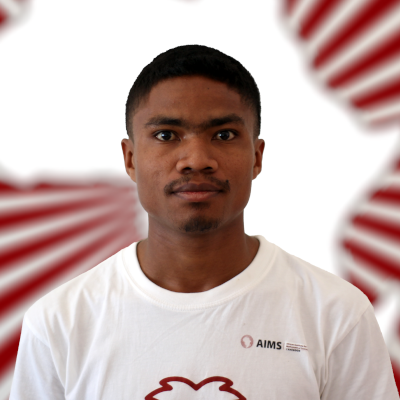
\includegraphics[scale=0.25]{img.png}};
			\draw[line width=3pt] (0,0) circle (1.5cm);
		\end{tikzpicture}
	\end{minipage}

\section{Summary}
\begin{adjustwidth}{\parindent}{\parindent}
	I am an enthusiastic problem-solver with a deep passion for mathematics and computer science. I enjoy learning and tackling challenges that require me to apply my interpersonal skills and technical know-how, as well as those that provide opportunities for personal growth. Moreover, I am always ready to face any challenges. I am dynamic, creative and flexible.
\end{adjustwidth}
\section{Education}
\subsection{Acdemic}
\begin{itemize}
	\item[\faGraduationCap] \cvEducEntry{MSc. in Machine Learning Artificial Intelligence}
	{Jan. 2024 -- Now}
	{Stellenbosch University}
	{Stellenbosch, South Africa}{}{}

	\item[\faGraduationCap]\cvEducEntry{MSc. in Mathematics and Applications -- Fundamental Mathematics}
	{2019 -- 2023}{Faculty of Science, University of Fianarantsoa}
	{Fianarantsoa, Madagascar}{\textbf{Relevant courses:} Algebraic Number theory, Cryptography, Enumerative Combinatorics and Algebra, Probability, Numerical Matrix Analysis, Distribution and PDE, Probability, Graph theory, Artificial intelligence.}
	{\textbf{Overall average:} 14.25/20}

	\item[\faGraduationCap] \cvEducEntry{Msc. in Mathematical Sciences -- Fundamental Sciences}{Sept. 2022 -- June 2023}{African Institute for Mathematical Science Cameroon}{Limb\'e Cameroon}{\textbf{Relevant courses:}
		Number Theory, Cryptography, Introduction to Algebraic Geometry, Numerical Optimization, Stochastic Analysis, Numerical Analysis With Python, Introduction to Quantum Information Theory, Statistical and Data Science problem Solving.}{
		\textbf{CGPA:} 3.52/4}

	\item[\faGraduationCap] \cvEducEntry{Bsc. in Mathematics and Application -- Fundamental Mathematics}{2015 -- 2019}{Faculty of Science, University of Fianarantsoa}{Fianarantsoa, Madagascar}{
		\textbf{Relevant courses:} General and Linear algebra, Geometry, Analysis, Topology, Algorithm, Differential Calculus, Measure and Integration.}
		{\textbf{Overall average:} 14.83/20}

	\item[\faGraduationCap] \cvEducEntry{Baccalaureate in Technology in Industrial Engineering}{2012 -- 2015}{Technical High School Beravina Fianarantsoa}{Fianarantsoa, Madagascar}{\textbf{Overall average:} 13.08/20}{}{}
\end{itemize}
\subsection{Extracuricular}
\begin{itemize}
	\item \cvEducEntry{Business Management}{Jully 2023 - August 2023}{ESMT Berlin, II Africa, IIP}{Limbe, Cameroon}{}{}
	\item \cvEducEntry{Back-end developer}{January 2022 - Jully 2022}{SAYNA \& OIF: DCLIC Program 1.0}{Fianarantsoa, Madagascar}{}{}
	\item \cvEducEntry{Probabilistic and statistical modeling in epidemiology and environment}{2021}{CIMPA}{Fianarantsoa, Madagascar}{}{}
\end{itemize}
\section{Publication and Talk}
\begin{itemize}
	\item[\faBook] Florian Luca and Jean Lucien Randrianantenaina, ``There Is No Carmichael Number of the Form $2^np^2+1$ with $p$ prime'', INTEGER, Volume 23 (2023).

	\item[\faComment*] Talk at AIMS Cameroon,  2023: ``Fermat last theorem, with n=4''
	Presented to AIMS Cameroon students. Supervised by Prof. Dr Hans Georg R\"{u}ck, Universität Kassel.
\end{itemize}
\section{Skills}
\begin{minipage}[H][4.3cm][t]{.5\linewidth}
	\begin{itemize}
			\skillEntry{Programming Languages}{Python, R, JavaScript, SageMath}
			\skillEntry{Database}{Sqlite3, MySQL}
			\skillEntry{Web Programming}{HTML5, CSS3}
			\skillEntry{Version Control}{Git/GitHub}
	\end{itemize}
\end{minipage}\begin{minipage}[H][4.3cm][t]{.4\linewidth}
	\begin{itemize}
			\languageEntry{Language}{English (Intermediate)}{French (Advanced)}{Malagasy (Native)}
			\skillEntry{Framework/Library/Runtime}{Numpy, Scipy, Sympy, Matplotlib, Pandas, Scikit-Learn, Tkinter, Tensorflow, OpenCV, Django, Flask, ReactJs, Bootstrap, NodeJs}
			\skillEntry{Others}{\LaTeX, Word, Excel, PowerPoint, GIMP, InkScape}
	\end{itemize}
\end{minipage}
\section{Personal Projects}
\begin{itemize}
	\item[\faCode]\projectentry{MK-Forum}{Continuous Project}{ Python, Django, Javascript, HTML, CSS/Bootstrap4, MathJax}{Creation of a forum dedicated to mathematics, developed using HTML, CSS/Bootstrap, and JS for the front end; Python/Django and MySQL for the back end. This project includes user account management, posts, comments, and a voting system.}

	%%%%%%%%
	\item[\faCode]\projectentry{FCryptos}{2023}{Python, Tkinter}{Implementation of cryptography methods with Python: Shift cypher, Vingenere cypher, SPN, RSA, and ENIGMA machine.}
	%%%%%%%%%%%%%%%
	\item[\faGamepad]\projectentry{Unbeatable TicTacToe}{2022}{ Javascript, HTML, CSS/Bootstrap}{Tic-Tac-Toe game created with HTML, CSS and JavaScript, and features an
		automated computer player that uses a combination of random placement
		and min-max algorithm to make each move depending on the chosen level.}
	%%%%%%%%%%%%%%%%%%%%%%%%%%%%%%
	\item[\faGamepad]\projectentry{Pendu Malagasy}{2022}{ Python, TKinter}{A Malagasy version of the game Hangman, built with Python3/TKinter.}
	%%%%%%%%%%%%%%%%%%%%%%
	\item[\faCode]\projectentry{Belllman Kalaba}{2021}{ Python, Tkinter}{A graphical interface for the algorithm of Bellman-Kalaba (shortest path)
		made with Python3/TKinter.}
\end{itemize}
\section{CERTIFICATIONS}
\begin{itemize}
	\item[\faCertificate] Hello-Elton: Communication, Positive Attitude, Self-awareness.
	\item[\faCertificate] PIF-TIC: Leadership, Social organization
\end{itemize}
\section{Prizes/Awards/Scholarships}
\begin{itemize}
	\item AIMS ESMT Industry Immersion Program (IIP) Scholarship, July 2023
	\item Fully Funded Master's Program at the African Institute for Mathematical Sciences (AIMS), sponsored by the Mastercard Foundation in Cameroon, 2022-2023
	\item Fully Funded D-CLIC 1.0 Program in 2022, offered by the International Organization of La Francophonie (OIF) and SAYNA
\end{itemize}
\end{document}